\documentclass{standalone}

\usepackage{ tikz }
\usetikzlibrary{automata, positioning, arrows}

\newcommand{\trs}[2]{#1 \,|\, #2}

\begin{document}
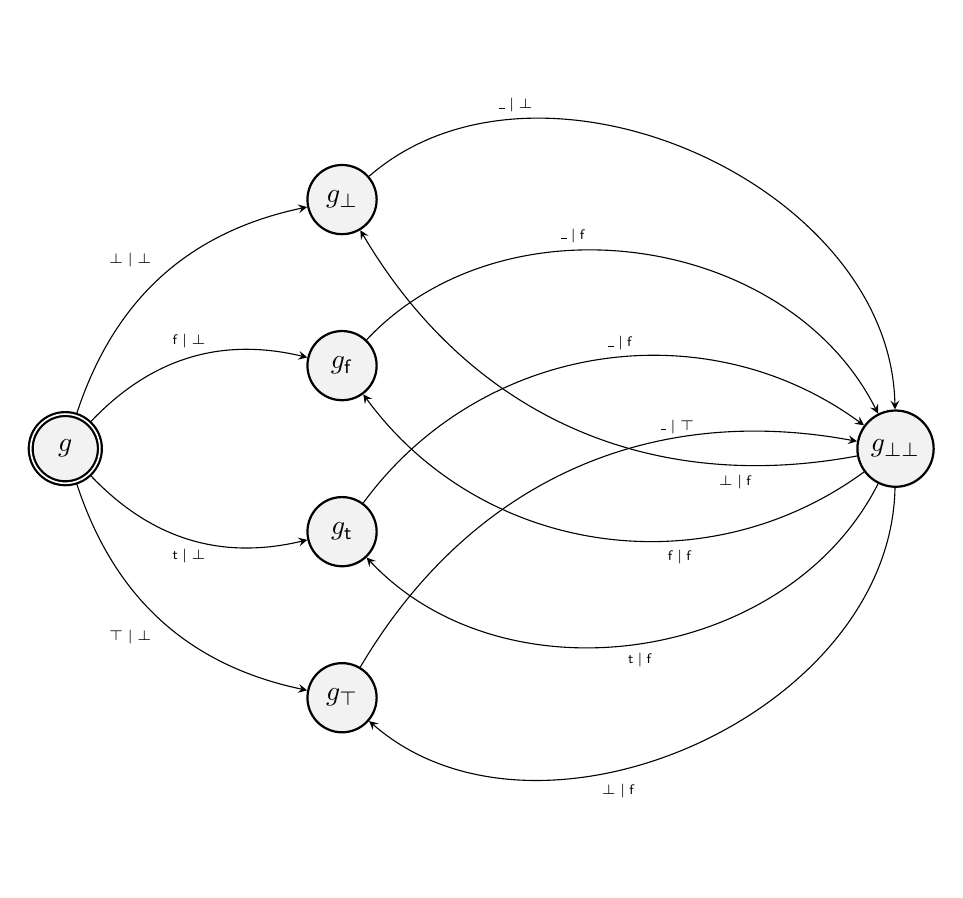
\begin{tikzpicture}[->, >=stealth, node distance=3cm, every state/.style={thick, fill=gray!10}, initial text=$ $, every edge/.append style={font=\tiny}, yscale=-1, x=100pt, y=30pt]
    \node[state, accepting] (s0) at (0,0) {\(g\)};
    \node[state] (s1) at (1,-3) {\(g_\bot\)};
    \node[state] (s2) at (1,-1) {\(g_\mathsf{f}\)};
    \node[state] (s3) at (1,1) {\(g_\mathsf{t}\)};
    \node[state] (s4) at (1,3) {\(g_\top\)};
    \node[state] (s5) at (3,0) {\(g_{\bot\bot}\)};

    \draw (s0) edge[bend right, above left] node{\(\trs{\bot}{\bot}\)} (s1);
    \draw (s0) edge[bend right, above] node{\(\trs{\mathsf{f}}{\bot}\)} (s2);
    \draw (s0) edge[bend left, below] node{\(\trs{\mathsf{t}}{\bot}\)} (s3);
    \draw (s0) edge[bend left, below left] node{\(\trs{\top}{\bot}\)} (s4);

    \draw (s1) edge[bend right=65, above right, pos=0.2] node{\(\trs{\_}{\bot}\)} (s5);
    \draw (s2) edge[bend right=55, above right, pos=0.35] node{\(\trs{\_}{\mathsf{f}}\)} (s5);
    \draw (s3) edge[bend right=45, above right, pos=0.5] node{\(\trs{\_}{\mathsf{f}}\)} (s5);
    \draw (s4) edge[bend right=35, above right, pos=0.65] node{\(\trs{\_}{\top}\)} (s5);

    \draw (s5) edge[bend right=35, below, pos=0.2] node{\(\trs{\bot}{\mathsf{f}}\)} (s1);
    \draw (s5) edge[bend right=45, below, pos=0.35] node{\(\trs{\mathsf{f}}{\mathsf{f}}\)} (s2);
    \draw (s5) edge[bend right=55, below, pos=0.5] node{\(\trs{\mathsf{t}}{\mathsf{f}}\)} (s3);
    \draw (s5) edge[bend right=65, below right, pos=0.65] node{\(\trs{\bot}{\mathsf{f}}\)} (s4);
\end{tikzpicture}
\end{document}